\matlab is a popular numeric programming language, used by millions of
scientists, engineers and students worldwide\cite{MatlabGrowth}.  \matlab
programmers appreciate the high-level matrix operators,  the fact that
variables and types do not need to be declared, the large number of library and
builtin functions available, and the interactive style of program development
available through the IDE and the interpreter-style read-eval-print loop.
However, even though \matlab programmers appreciate all of the features that
enable rapid prototyping,  they often have other ultimate goals.  Frequently
their computations are quite computationally intensive and they really want an
efficient implementation.  Programmers also often want to integrate their
\matlab program into existing static systems.  As just one example, one of our
users wanted to generate {\sc FORTRAN} code that can be plugged into a weather
simulation environment.    

This thesis addresses the problem of how to provide the bridge between
the dynamic realities of \matlab and the ultimate goal of wanting
efficient and static programs in languages like {\sc FORTRAN}.  It is
not realistic to support all the \matlab features, but our goal is to
define and provide support for a very large subset of \matlab which
includes dynamic typing, support of the \matlab function lookup
semantics, variable numbers of input and output arguments, support for
a variety of \matlab data types including arrays, cell arrays and
structs, and support for function handles and lambda expressions.

Providing this bridge presents two main challenges.  The first is that \matlab
is actually quite a complex language which has evolved over many years and
which has non-standard type rules and function lookup semantics.  The second
major challenge is properly dealing with the large number of builtin and
library functions,  which have also been developed over time and which
sometimes have unexpected or irregular behavior. 

\begin{figure}[htbp]
\begin{center}
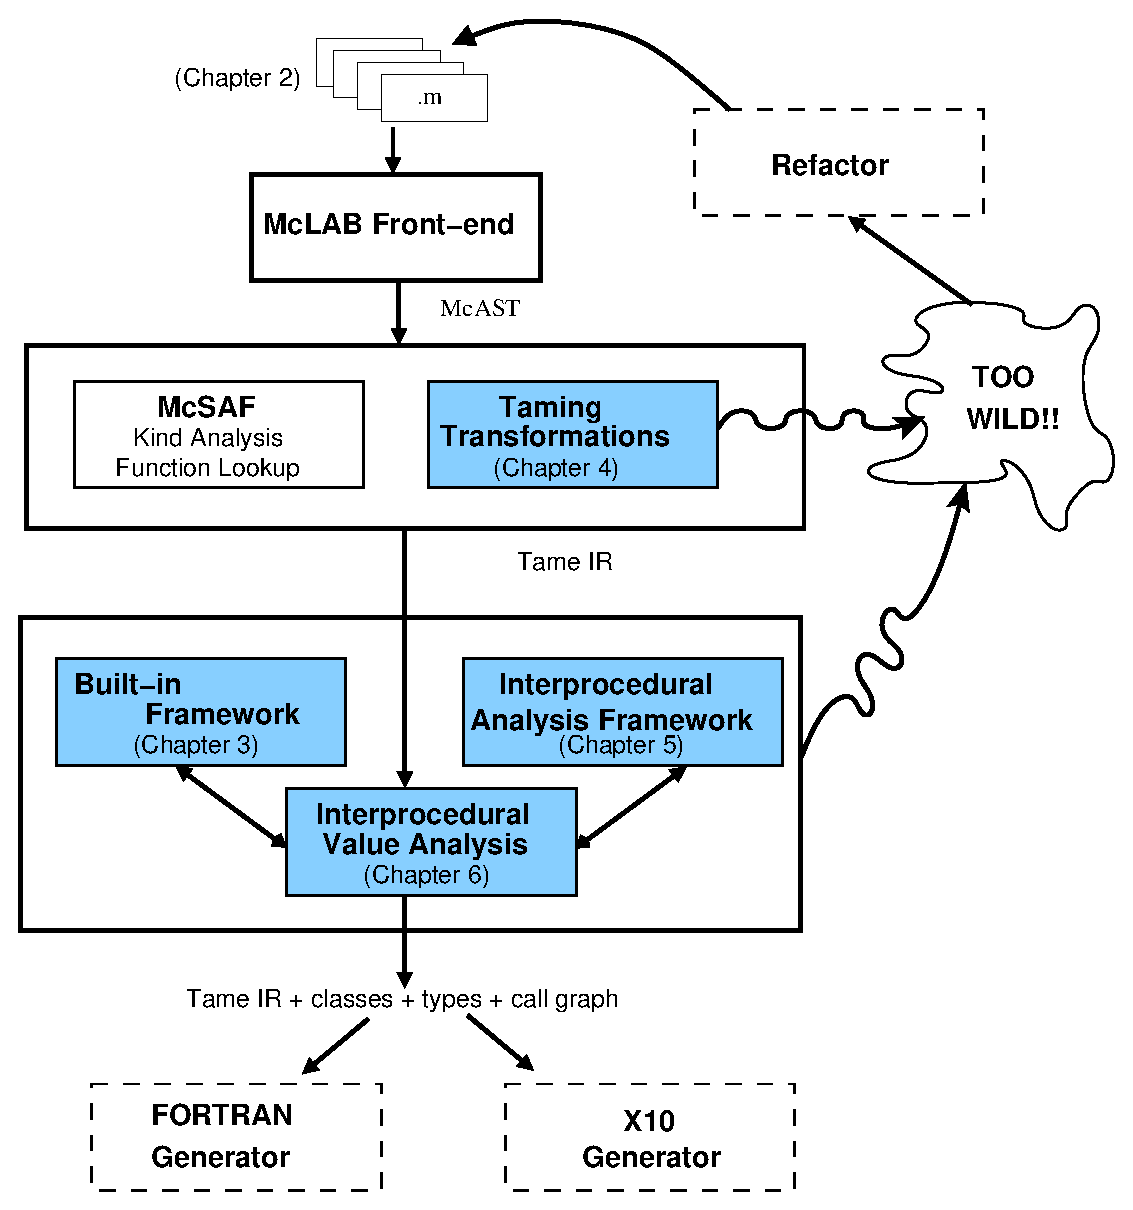
\includegraphics[width=3.5in]{Figures/overview.eps}
\caption[Overview of the \matlab Tamer]{Overview
of our \matlab Tamer.  The shaded boxes indicate the components
presented in this thesis.  The other solid boxes correspond to
existing \mclab tools we use, and the dashed boxes correspond to
ongoing projects which are using the results of this
thesis.}\label{Fig:Overview}
\end{center}
\end{figure}

Our solution is an open-source extensible objected-oriented framework,
implemented in Java, as presented in \figref{Fig:Overview}.   The overall
goal of the system is to take \matlab programs as input and produce output
which is suitable for static compilation, a process that we call
\textit{Taming} \matlab.   Given a \texttt{.m} file as input, which is the
entry point, the \matlab Tamer produces as output: (1) a Tame
IR \rednote{(intermediate representation)} for all functions (both user
and library) which are reachable from the entry point, (2) a complete
call graph, and (3) an estimation of classes/types for all variables.

There are some features in \matlab that are simply too wild to handle, and so
our system will reject programs using those features, and the user will need to
refactor their program to eliminate that feature.   Thus, another important
goal in our work is to define as large as possible subset of \matlab that can
be tamed without user intervention. 

\section{Contributions}

The main contributions of this thesis are as follows.

\begin{itemize}
\item We present an overall design and implementation for the \matlab Tamer,
an extensible object-oriented framework
which provides the bridge between the dynamic \matlab language and a static back-end
compiler. 

\item We describe the key features of \matlab necessary for compiler developers
and for tool writers to understand \matlab and the analyses in this thesis.  We hope
that by carefully explaining these ideas, we can enable other researchers
to also work on static tools for \matlab.  Our discussion of \matlab features
also motivates our choice of the subset of \matlab that we aim to tame. 

\item We provide a principled approach to understanding, grouping, and
analyzing the large number of \matlab builtin functions.

\item We developed extensions to the \mcsaf\cite{JesseThesis} framework to support a lower-level
and more specialized Tame IR, suitable for back-end static code generation.

\item We present an interprocedural flow analysis framework that allows
 extending intraprocedural analysis written for the \mcsaf framework to
 analyze whole programs.
 
\item We present an interprocedural flow analysis framework that computes both
abstract values and the complete call graph.  This flow analysis
provides an object-oriented approach which allows for extension and
refinement of the abstract value representations.

\end{itemize}


\section{Thesis Outline}
This thesis is divided into \ref{chap:Conclusions} chapters, including this one, which are structured as follows.

\chapref{chap:MATLAB} introduces key \matlab features,
showing some of the challenges of static compilation.
\chapref{chap:Builtin} describes our
approach to dealing with \matlab builtin functions, starting with some
examination of which builtin functions are relevant, and how they
behave.
\chapref{chap:TameIR} presents the Tame IR and
transformations, including how these were integrated with the existing
analysis framework.
\chapref{chap:inter} describes our interprocedural analysis framework.
\chapref{chap:ValueAnalysis} explains our 
extensible and modular interprocedural value analysis and how it
constructs complete callgraphs. We also show some results of running
this analysis on a set of benchmarks.
\chapref{chap:Related} provides an overview of related work and
\chapref{chap:Conclusions} concludes.
